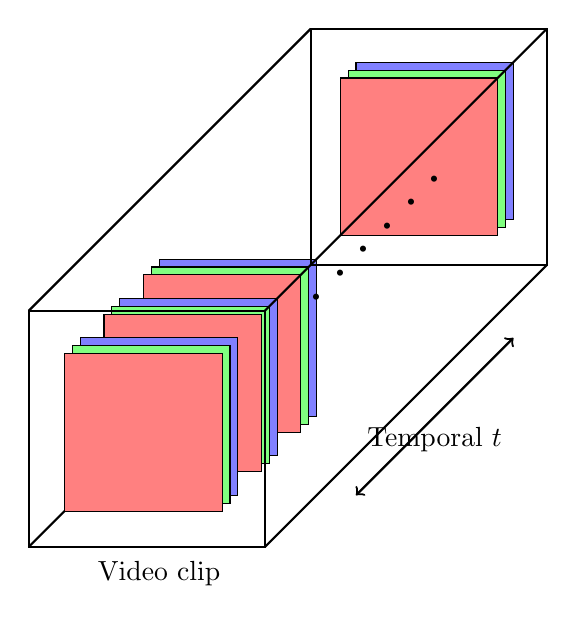
\begin{tikzpicture}
    % 3D Cube - we want to draw some of the cube edges below the frames
    % variables
    \def\cubeWidth{3}
    \def\cubeHeight{3}
    % \def\cubeDepth{8}

    % Cube points
    \coordinate (A) at (0, 0, -5);
    \coordinate (B) at (\cubeWidth, 0, -5);
    \coordinate (C) at (\cubeWidth, \cubeHeight, -5);
    \coordinate (D) at (0, \cubeHeight, -5);
    \coordinate (E) at (-0.5, -0.5, 3);
    \coordinate (F) at (\cubeWidth - 0.5, -0.5, 3);
    \coordinate (G) at (\cubeWidth - 0.5, \cubeHeight - 0.5, 3);
    \coordinate (H) at (-0.5, \cubeHeight - 0.5, 3);

    % Draw cube edges that are below the frames
    \draw[thick] (A) -- (E);

    \def\width{2}
    \def\height{2}
    \def\shift{0.1} % Shift for the green and red channels

    \def\xshift{-0.5}  % Shift in the x direction for duplication
    \def\yshift{-0.5}  % Shift in the y direction for duplication
    \def\lastrectxshift{\xshift * -5} % Last image should be shifted more because of three dots
    \def\lastrectyshift{\yshift * -5} % Last image should be shifted more because of three dots
    \def\dotstartx{2}  % Starting x position for the dots
    \def\dotstarty{1.5}  % Starting y position for the dots
    \def\dotshift{0.3}  % Shift for the dots


    % First rectangle
    \draw[fill=blue!50] (0, 0) rectangle (\width, \height);
    \draw[fill=green!50] (-\shift, -\shift) rectangle (\width-\shift, \height-\shift);
    \draw[fill=red!50] (-2*\shift, -2*\shift) rectangle (\width-2*\shift, \height-2*\shift);

    % Second rectangle
    \draw[fill=blue!50] (\xshift, \yshift) rectangle (\xshift+\width, \yshift+\height);
    \draw[fill=green!50] (\xshift-\shift, \yshift-\shift) rectangle (\xshift+\width-\shift, \yshift+\height-\shift);
    \draw[fill=red!50] (\xshift-2*\shift, \yshift-2*\shift) rectangle (\xshift+\width-2*\shift, \yshift+\height-2*\shift);

    % Third rectangle
    \draw[fill=blue!50] (2*\xshift, 2*\yshift) rectangle (2*\xshift+\width, 2*\yshift+\height);
    \draw[fill=green!50] (2*\xshift-\shift, 2*\yshift-\shift) rectangle (2*\xshift+\width-\shift, 2*\yshift+\height-\shift);
    \draw[fill=red!50] (2*\xshift-2*\shift, 2*\yshift-2*\shift) rectangle (2*\xshift+\width-2*\shift, 2*\yshift+\height-2*\shift);

    % Fourth rectangle
    \draw[fill=blue!50] (\lastrectxshift, \lastrectyshift) rectangle (\lastrectxshift+\width, \lastrectyshift+\height);
    \draw[fill=green!50] (\lastrectxshift-\shift, \lastrectyshift-\shift) rectangle (\lastrectxshift+\width-\shift, \lastrectyshift+\height-\shift);
    \draw[fill=red!50] (\lastrectxshift-2*\shift, \lastrectyshift-2*\shift) rectangle (\lastrectxshift+\width-2*\shift, \lastrectyshift+\height-2*\shift);


    % Dots
    \node at (\dotstartx, \dotstarty) {\huge$\cdot$};
    \node at (\dotstartx + \dotshift, \dotstarty + \dotshift) {\huge$\cdot$};
    \node at (\dotstartx + \dotshift*2, \dotstarty + 2*\dotshift) {\huge$\cdot$};
    \node at (\dotstartx + \dotshift*3, \dotstarty + 3*\dotshift) {\huge$\cdot$};
    \node at (\dotstartx + \dotshift*4, \dotstarty + 4*\dotshift) {\huge$\cdot$};
    \node at (\dotstartx + \dotshift*5, \dotstarty + 5*\dotshift) {\huge$\cdot$};

    % Arrow
    \draw[<->, thick] (2.5, -1) -- (4.5, 1) node[midway, below] {Temporal $t$};







    % Draw the rest of the cube
    \draw[thick] (A) -- (B) -- (C) -- (D) -- cycle;
    \draw[thick] (E) -- (F) -- (G) -- (H) -- cycle;
    \draw[thick] (B) -- (F);
    \draw[thick] (C) -- (G);
    \draw[thick] (D) -- (H);

    % Draw clip text
    \node at (0, -2) {Video clip};

    

\end{tikzpicture}
